\documentclass{gtpart}
\usepackage{amsmath,amssymb,amsthm,stmaryrd}
\usepackage[all]{xy}
\usepackage{tikz}
\usepackage{url}
%\usepackage{setspace}
%\doublespacing

\title{The power operation structure on the $K(1)$-localization of $E_2$}
\author{Yifei Zhu}
\givenname{Yifei}
\surname{Zhu}
%\address{Department of Mathematics\\University of Minnesota\\Minneapolis, MN 55455\\USA}
%\email{zyf@umn.edu}

%\subject{primary}{msc2000}{55P99}
%\subject{secondary}{msc2000}{55Q99}

%\bibliographystyle{gtart}
\parskip 0.7pc
\parindent 0pt

\newtheorem{thm}{Theorem}
\newtheorem{cor}[thm]{Corollary}
\newtheorem{prop}[thm]{Proposition}
\newtheorem{lem}[thm]{Lemma}
\theoremstyle{definition}
\newtheorem{defn}[thm]{Definition}
\theoremstyle{remark}
\newtheorem{rmk}[thm]{Remark}
\newtheorem{exam}[thm]{Example}
\newtheorem{case}[thm]{Case}
\newtheorem{slogan}[thm]{Slogan}
\newtheorem{ques}[thm]{Question}

\def\co{\colon\thinspace}
\newcommand{\mb}[1]{\mathbb{#1}}
\newcommand{\mf}[1]{\mathfrak{#1}}

\newcommand{\NB}[1]{{\bf (NB: #1)}}

\newcommand{\Ext}{\ensuremath{{\rm Ext}}}
\newcommand{\Coext}{\ensuremath{{\rm Coext}}}
\newcommand{\Hom}{\ensuremath{{\rm Hom}}}
\newcommand{\Tor}{\ensuremath{{\rm Tor}}}
\newcommand{\Ind}{\ensuremath{{\rm Ind}}}
\newcommand{\Res}{\ensuremath{{\rm Res}}}
\newcommand{\colim}{\ensuremath{\mathop{\rm colim}}}
\newcommand{\hocolim}{\ensuremath{\mathop{\rm hocolim}}}
\newcommand{\holim}{\ensuremath{\mathop{\rm holim}}}
\newcommand{\overto}{\mathop\rightarrow}
\newcommand{\overfrom}{\mathop\leftarrow}
\newcommand{\into}{\mathop\hookrightarrow}
\newcommand{\onto}{\mathop\twoheadrightarrow}
\newcommand{\longoverto}{\mathop{\longrightarrow}}
\newcommand{\Irr}{\ensuremath{\mathop{\rm Irr}}}
\newcommand{\Rep}{\ensuremath{\mathop{\rm Rep}}}
\newcommand{\Map}{\ensuremath{{\rm Map}}}
\newcommand{\GL}{{\rm GL}}
\newcommand{\Uni}{{\rm U}}
\newcommand{\BU}{{\rm BU}}
\newcommand{\Sp}{{\cal S}p}
\newcommand{\Sym}{{\rm Sym}}
\newcommand{\thh}{{\rm thh}}
\newcommand{\TAF}{{\rm TAF}}
\newcommand{\TAQ}{{\rm TAQ}}
\newcommand{\End}{{\rm End}}
\newcommand{\Aut}{{\rm Aut}}
\newcommand{\md}{{\rm mod}}
\newcommand{\As}{{\cal A}s}
\newcommand{\LT}{{\rm LT}}
\newcommand{\Spec}{{\rm Spec}}
\newcommand{\Spf}{{\rm Spf}}
\newcommand{\tmf}{{\rm tmf}}
\newcommand{\eo}{{\rm eo}}
\newcommand{\TMF}{{\rm TMF}}
\newcommand{\Ell}{{\cal E}ll}
\newcommand{\Lie}{{\rm Lie}}
\newcommand{\Sh}{{\rm Sh}}
\newcommand{\HF}{{\rm H}{\mb F}}
\newcommand{\cF}{\overline {\mb F}}
\newcommand{\cQ}{\overline {\mb Q}}

\newcommand{\eilm}[1]{\ensuremath{{\mb H} #1}}
\newcommand{\smsh}[1]{\ensuremath{\mathop{\wedge}_{#1}}}
\newcommand{\tens}[1]{\ensuremath{\mathop{\otimes}_{#1}}}
\newcommand{\susp}{\ensuremath{\Sigma}}
\newcommand{\mapset}[3]{\ensuremath{\left[#2,#3\right]_{#1}}}
\newcommand{\form}[2]{\ensuremath{\left\langle#1,#2\right\rangle}}
\newcommand{\bilin}[2]{\ensuremath{\left(#1,#2\right)}}
\newcommand{\comp}[1]{\ensuremath{#1^\wedge}}
\newcommand{\loca}[3]{\ensuremath{L^{#1}_{#2}(#3)}}
\newcommand{\tc}[3]{\ensuremath{\Omega_{#2 / #1}^{#3}}}
\newcommand{\atc}[3]{\ensuremath{\L_{#2 / #1}^{#3}}}

\newcommand{\xym}[1]{
\vskip 0.7pc
\centerline{\xymatrix{#1}}
\vskip 0.7pc
}

\newcommand{\DL}{{\rm DL}}
\newcommand{\CA}{{\cal A}}
\newcommand{\Mod}{{\rm Mod}}
\newcommand{\Alg}{{\rm Alg}}
\newcommand{\Frob}{{\rm Frob}}
\newcommand{\CO}{{\cal O}}
\newcommand{\DF}{{{\rm DefFrob}_\Gamma}}
\newcommand{\Model}{{\rm Model}}
\newcommand{\Gm}{{{\mb G}_m}}
\newcommand*{\longhookrightarrow}{\ensuremath{\lhook\joinrel\relbar\joinrel\rightarrow}}

\begin{document}

\begin{abstract}
 Dyer-Lashof theories organize power operations in cohomology.  We give an overview of the structure of the Dyer-Lashof theories 
 associated to Morava $E$-theories, and to their $K(1)$-localizations.  
 When the $E$-theory is an elliptic cohomology theory, this structure enables us to compute power operations by calculation with 
 elliptic curves.  
\end{abstract}

\maketitle
\section{Introduction}
\label{sec:intro}


The study of cohomology operations has become central to algebraic 
topology since the 1950s, with applications to solving problems such as 
vector fields on spheres, and the non-existence of elements of Hopf 
invariant one.  This latter problem has impact on the author most 
recently felt when he tried to answer a question raised by students in a 
calculus class (the interested reader might see \cite[theorem II]{massey}).  

Among the operations involved in these applications, the Steenrod operations ${\rm Sq}^i$ in ordinary cohomology, 
and the Adams operations $\psi^k$ in $K$-theory are examples of {\em power operations}.  
In this paper we study power operations in Morava $E$-theories.  Here is 
an outline.  

In this section we introduce preliminary definitions, in 
particular, the Dyer-Lashof theory $\DL_{E_*}$ associated to a Morava 
$E$-theory $E_*$.  

In section \ref{sec:at2ec} we ``translate'' from $\DL_{E_*}$ and related 
categories, to categories arising from the formal group and its finite flat subgroups 
associated to $E_*$.  This ``bridge'' is the foundation 
of our discussion, so that later we can study the structure of one side by doing calculation on the other side.  

In section \ref{sec:K(1)} we describe power operations in the $K(1)$-local setting where the structure is relatively simple.  

Section \ref{sec:p3} contains calculations of power 
operations for a specific Morava $E$-theory spectrum and its 
$K(1)$-localization, at the prime 3.  Thanks to the connection in section \ref{sec:at2ec}, we work with elliptic curves as concrete objects, following a recipe in hope of 
generalizing our computation to larger primes.  


\subsection{Dyer-Lashof theories}
\label{subsec:DL}

One organizing principle for understanding the structure among cohomology operations 
is through the {\em algebraic theories} (due to Lawvere, cf. 
\cite{lawvere} and \cite[chapter 3]{borceux}).  We will have to begin with a 
collection of definitions and simple facts concerning algebraic theories, 
following precisely the discussion in \cite[sections 5--9]{lpo}.  
\begin{defn}
 An {\em (algebraic) theory} is a category $T$ with object set 
 $\{T^0,T^1,T^2,...\}$, together with a canonical map 
 $T^0 \to T^1$, and {\em projection maps} $\pi_i\co T^n \to T^1$ for all 
 $n \geq 1$, $1 \leq i \leq n$ such that $T(T^k,T^n) \xrightarrow{\pi_i} 
 \prod_{i=1}^n T(T^k,T^1)$ is a bijection for all $k$ and $n$, 
 i.e.\thinspace$T^n$ is isomorphic to the $n$-fold product of $T^1$.  
 
 A {\em morphism of theories} is a functor $\phi\co R \to T$ which 
 preserves the product structure of a theory, i.e.\thinspace$\phi(R^k) = 
 T^k$ and $\phi(R^k \stackrel{\pi_i}{\longrightarrow} R^1) = T^k 
 \stackrel{\pi_i}{\longrightarrow} T^1$.  
\end{defn}

\begin{defn}
 A {\em model} of $T$ is a functor $A\co T \to \rm{Set}$ which 
 preserves finite products.  
\end{defn}
It can be thought of as the underlying set $X = A(T^1)$ together with 
operations $\psi_f\co X^k \to X^n$ for each 
$f \in T(T^k,T^n)$.  In particular, a {\em free model} on $n$ generators 
is the model $F_T(n)$ defined by $F_T(n)(T^m) = T(T^n,T^m)$.  We write 
$\Model_T$ for the category of models of $T$.  For example, let $R$ be a 
commutative ring, and let $F$ be the full subcategory of the category of 
commutative $R$-algebras having as objects $\{F_0,F_1,F_2,...\}$, where 
$F_0 = R$ and $F_n = R[x_1,...,x_n]$ for $n \geq 1$.  We then have the 
theory of commutative $R$-algebras $C_R = F^{\rm op}$.  

\begin{defn}
 A {\em commutative operation theory} (COT) is a triple $(T,R,\phi)$ 
 consisting of a theory $T$, a commutative ring $R$, and a morphism 
 $\phi\co C_R \to T$ of theories, such that the induced functor 
 $\phi^*\co \Model_T \to \Model_{C_R}$ commutes with finite coproducts.  
\end{defn}
In other words, every $T$-model has an underlying structure of a 
commutative $R$-algebra, and coproducts in $\Model_T$ are computed by 
tensor products over $R$.  We write $R\{x_1,...,x_n\}$ for a free 
$T$-model on $n$ generators, and we have $R\{x_1,...,x_n\} \cong 
R\{x_1\} \otimes_R \cdots \otimes_R R\{x_n\}$.  

We next introduce grading to a theory.  
\begin{defn}
 Let $C$ be a fixed set $C$ of {\em colors}, and let ${\mb N}[C]$ be the 
 free commutative monoid on $C$.  A {\em $C$-graded theory} $T$ is a 
 category with object set $\{T^n\}_{n \in {\mb N}[C]}$, together with, 
 for each $n = \sum_{c \in C} n_c[c] \in {\mb N}[C]$, a specified 
 identification of $T^n$ with the product 
 $\prod_{c \in C} (T^{[c]})^{n_c}$.  
\end{defn}
In particular, given a $\mb Z$-graded theory $T$ and a graded-commutative 
ring $R$, we can define a graded COT as a triple $(T,R_*,\phi)$ similarly 
as above (the theory $C_{R_*}$ of graded-commutative $R_*$-algebras is 
equipped with the graded tensor product).  Given a $T$-model $A$, we write 
$A_c$ for the piece with grading $c$ of the model.  

For a graded COT $(T,R_*,\phi)$, and free models $R_*\{x\}$ and 
$R_*\{x_1,x_2\}$ with $|x| = |x_1| = |x_2| = c$, let ${\cal A}(c,d)$ 
be the set of elements $f \in R_*\{x\}_d = T(T^{[c]},T^{[d]})$ which are 
primitive under the comultiplication 
$R_*\{x\} \xrightarrow{x \mapsto x_1 + x_2} R_*\{x_1,x_2\}$.  Such 
$f \in {\cal A}(c,d)$ give rise to additive functions $A_c \to A_d$ 
natural in the model $A$, and in particular the element $x \in R_*\{x\}_c$ 
corresponds to the identity map on $A_c$.  Thus we obtain a category 
$\cal A$ of additive operations, whose object set is $\mb Z$, the set of 
colors of our graded COT.  

For example, let $T = O_{H{\mb F}_p}$ be the graded COT given by 
\[
 T(O_{H{\mb F}_p}^{[c_1]+\cdots+[c_m]},O_{H{\mb F}_p}^{[d_1]+\cdots+[d_n]}) 
 = [K({\mb F}_p,c_1) \times \cdots \times K({\mb F}_p,c_m), 
 K({\mb F}_p,d_1) \times \cdots \times K({\mb F}_p,d_n)],
\]
where we use homotopy classes of maps, and use the convention that 
$K({\mb F}_p,c) = *$ for $c<0$.  Then $\Model_{O_{H{\mb F}_p}}$ is the 
category of unstable algebras over the mod-$p$ Steenrod algebra.  
Moreover, ${\cal A}(c,d)$ is the set of additive operations 
$H^c(-;{\mb F}_p) \to H^d(-;{\mb F}_p)$; in particular, for $p=2$, these 
are linear combinations of monomials which are admissible composites of Steenrod 
operations having excess no more than $c$.  Cf. \cite[section 4.L]{at} for details.  

Having the COT describing cohomology operations on spaces, we next 
consider one describing operations on spectra.  

Let $S$ be the sphere 
spectrum, and $\Alg_S$ be the category of commutative $S$-algebras (cf. 
\cite{EKMM}).  Let $\mb P$ be the free $S$-algebra functor defined by 
\[
 {\mb P}(X) = \bigvee_{m \geq 0} {\mb P}^m(X) = \bigvee_{m \geq 0} 
 X^{\wedge m}/\Sigma_m,
\]
and let ${\mb P}_R$ be the free $R$-algebra functor 
defined similarly using the smash product over $R$.  These functors 
descend to homotopy categories.  
\begin{defn}
 Given a commutative $S$-algebra $R$, the {\em Dyer-Lashof theory} 
 $\DL_R$ is the $\mb Z$-graded theory $T$ defined by 
 \[
  T(T^{[c_1]+\cdots+[c_m]},T^{[d_1]+\cdots+[d_n]}) = h\Alg_R 
  \Big({\mb P}_R \big(R \wedge (S^{d_1} \vee \cdots \vee S^{d_n}) \big), 
  {\mb P}_R \big(R \wedge (S^{c_1} \vee \cdots \vee S^{c_m}) \big) \Big).
 \]
\end{defn}
In the homotopy category, we can identify ${\mb P}^m (S^c)$ with $B\Sigma_m^{cV_m}$ 
which is the Thom spectrum of a virtual bundle ($V_m = {\mb R}^m$ is equipped with the $\Sigma_m$-action given by 
permuting coordinates, and $c \in {\mb Z}$).  The free theories are given by 
\[
 F_T([c_1]+\cdots+[c_m])_{[d]} = \pi_d {\mb P}_R  \big( R \wedge (S^{c_1} 
 \vee \cdots \vee S^{c_m}) \big) = \pi_d \Big( R \wedge 
 \big({\mb P}(S^{c_1}) \vee \cdots \vee {\mb P}(S^{c_m})\big) \Big).
\]
Moreover, if $\pi_*R\wedge{\mb P}(S^c)$ are flat as left 
$\pi_*R$-modules, $\DL_R$ turns out to be a COT (cf. \cite[lemma 7.5]{lpo}).  

The significance of $\DL_R$ is 
that it describes all homotopy operations on commutative $R$-algebras: 
\[
 \DL_R([c],[d]) = h\Alg_R \big( {\mb P}_R(R \wedge S^d), 
 {\mb P}_R(R \wedge S^c) \big) = \{\pi_c(-) \to \pi_d(-)\}.
\]
For example, if $R$ is a ring (no longer a spectrum) containing 
${\mb F}_2$ and $HR$ is the corresponding Eilenberg-Mac~Lane spectrum, there is a complete description of the COT $\DL_{HR}$.  
A $\DL_{HR}$-model is a graded commutative $R$-algebra $A_*$, 
equipped with functions $Q^s\co A_c \to A_{c+s}$ for all 
$s, c \in {\mb Z}$, satisfying a set of properties, e.g.\thinspace{t}he 
Cartan formula and the Adem relations.  Cf. \cite[section 10]{lpo} for details.  


\subsection{Dyer-Lashof theories associated to Morava $E$-theories}
\label{subsec:DL}

One organizing principle for understanding large-scale phenomena in 
homotopy theory is through the {\em chromatic filtration} (cf. 
\cite{tafoverview} and \cite[section 17]{coctalos}) which corresponds to a stratification 
of the moduli stack of formal groups into layers according to height.  
For complex oriented cohomology theories, the formal groups come about in 
terms of formal group laws which express the first Chern class of the 
tensor product of two line bundles in terms of the first Chern classes of 
the individual line bundles.  

For each formal group law $F$ of height $n<\infty$ over a perfect field 
$k$ of characteristic $p>0$, the Lubin-Tate ring $\LT(k,F) = 
{\mb W}k \llbracket v_1,...,v_{n-1} \rrbracket$ is universal among 
complete local rings with residue field $k$ carrying a formal group law 
whose reduction to $k$ is $F$.  There is an $E_\infty$ ring spectrum 
$E_n(k,F)$ whose homotopy groups are $\LT(k,F)[v^{\pm1}]$ with $|v| = 2$.  
This is the {\em Morava $E$-theory} spectrum (associated to $k$ and $F$).  
One can study specific layers in the chromatic filtration through 
Bousfield localization (cf. \cite[lectures 20--23]{252x}).  For example, 
the $K(1)$-localization of $E_2$ is the localization to height 1 of a 
certain Morava $E$-theory of height 2; the open substack of heights less 
than or equal to 2 is where {\em elliptic cohomology theories} 
(cf. \cite{survey}) are concentrated.  

Given a Morava $E$-theory $E_*$, there is an associated Dyer-Lashof 
theory $\DL_{E_*}$ describing all cohomology operations.  It is 
defined similarly as above, except that we need to apply a certain 
localization to have good values of $E_* B\Sigma_m$ (which is mostly 
torsion for a general ring spectrum $E$) (cf. \cite[section 3]{strickland} and 
\cite[section 8]{hoveystrickland}).  In particular the free model on one 
generator is $E_*\{x_c\} = 
\bigoplus_{m \geq 0} E_*^\wedge (B\Sigma_m^{cV_m})$, where the completed 
theory $E_*^\wedge (-)$ reflects the localization.  

As is explained at the beginning of \cite{Andu}, we hope to learn about 
the conjectural geometry of the theories $E_n$ by examining cohomology 
operations -- in particular, power operations -- along the lines of 
ordinary rational homology or $K$-theory (which are the initial cases 
$E_0$ and $E_1$).  


\section{The structure of power operations}
\label{sec:at2ec}


Let $E_*$ be the Morava $E$-theory associated to a formal group $\Gamma$ 
of height $n<\infty$ over a perfect field $k$ of characteristic $p>0$.  
Based on knowledge of the spectrum $E$, we study the structure of 
$\DL_{E_*}$, the $\mb Z$-graded Dyer-Lashof theory describing all homotopy operations on commutative $E$-algebras.  We 
restrict our attention to the degree 0 part $\DL_{E_0}$.  The main input 
comes from deformations of Frobenius, which we discuss below.  In 
particular, when the $E$-theory is an elliptic cohomology theory, deformations of Frobenius are parametrized by 
finite flat subgroups of the formal group of the associated elliptic curve, 
and thus we may study the operations by calculation with elliptic curves.  

This section is largely a summary of some of the results in \cite[section 16]{lpo} 
and \cite[sections 3 and 4]{h2p2}.  Cf. \cite{slides} for an exposition of related topics.  

\subsection{Identifications of categories}
\label{subsec:id}

First we consider additive operations.  

Let $\CA$ be the set of 
additive elements in the free $\DL_{E_0}$-model on one generator 
$E_0\{x\} = \bigoplus_{m \geq 0} E_0^\wedge B\Sigma_m$.  Write 
$\CA_{[m]} \subset E_0^\wedge B\Sigma_m$ for the summand, and write 
$\CA_r = \CA_{[p^r]}$.  It turns out that $\CA_{[m]} = 0$ unless 
$m = p^r$ for some $r$ (cf. \cite[lemma 8.10]{strickland}).  Thus 
$\CA = \bigoplus_{r \geq 0} \CA_r$ is an associative (not necessarily 
commutative) graded ring with respect to the product given by ``composition 
of operations'', with the unit element given by the generator 
$x \in E_0\{x\}$ representing the identity operation.  Moreover, the 
category $\Mod_\CA$ of left $\CA$-modules naturally admits a tensor 
product which makes it into a symmetric monoidal category (cf. \cite[proposition 7.6]{lpo}).  

We formulate a category equivalent to $\Mod_\CA$, which is specific to 
Morava $E$-theories, using deformations of Frobenius.  

Let $R$ be a 
complete local ring containing ${\mb F}_p$ with maximal ideal $\mf m$.  Given an $R$-algebra $A$, let $\Frob^*\co \sigma^*A \to A$ be the 
map of $R$-algebras which fits into the diagram 
\begin{center}
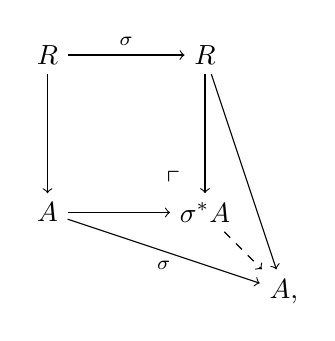
\begin{tikzpicture}
	\node (LT) at (0, 3) {$R$};
        \node (LB) at (0, 1) {$A$};
	\node (RT) at (2, 3) {$R$};
	\node (RB) at (2, 1) {$\sigma^*A$};
	\node (RB0) at (3, 0) {$A$,};
	\node at (1.6, 1.4) {$\ulcorner$};
	\draw [->] (LT) -- (LB);
	\draw [->] (LT) -- node [above] {$\scriptstyle \sigma$} (RT);
        \draw [->] (LB) -- (RB);
	\draw [->] (LB) -- node [below] {$\scriptstyle \sigma$} (RB0);
	\draw [->] (RT) -- (RB);
	\draw [->] (RT) -- (RB0);
	\draw [->, dashed] (RB) -- (RB0);
\end{tikzpicture}
\end{center}
where $\sigma$ sends an element to its $p$'th power.  In particular, if 
$G$ is a formal group over $R$, there is an isogeny 
$\Frob\co G \to \sigma^*G$ of formal groups over $R$ defined by 
$\Frob^*\co \CO_{\sigma^*G} = \sigma^*\CO_G \to \CO_G$, 
$R \llbracket y \rrbracket \to R \llbracket x \rrbracket$ sending $y$ to 
$x^p$.  

A {\em deformation of $\Gamma$ to $R$} is a triple $(G,i,\alpha)$ 
consisting of a formal group $G$ over $R$, an inclusion 
$i\co k \to R/\mf m$ and an isomorphism $\alpha\co G_0 \to i^*\Gamma$ of 
formal groups over $R/\mf m$.  A {\em $\star$-isomorphism 
$(G,i,\alpha) \to (G',i',\alpha')$} is an isomorphism $\phi\co G \to G'$ 
of formal groups over $R$ such that $i' = i$ and 
$\alpha' \circ \phi_0 = \alpha$.  We define the {\em category of 
deformations of Frobenius over $R$} as follows.  
\begin{defn}
 Let $\DF(R)$ be the category whose objects are deformations of $\Gamma$ 
 to $R$, and whose morphisms are isogenies which are deformations of 
 Frobenius, i.e.\thinspace{a} morphism $(G,i,\alpha) \to (G',i',\alpha')$ 
 is an isogeny $\phi\co G \to G'$ such that $i' = \sigma^r \circ i$ and 
 $\alpha' \circ \phi_0 = \Frob^r \circ \alpha$ for some $r \geq 0$.  In 
 particular, when $r = 0$, $\phi$ is precisely a $\star$-isomorphism.  
\end{defn}

We then consider the category of sheaves of modules on $\DF = \{\DF(R)\}$.  
\begin{defn}
\label{def:mod}
 Define a category $\Mod_\DF$ as follows.  An object $\cal F$ of this 
 category consists of 
 \begin{enumerate}
  \item for each complete local ring $R$ containing ${\mb F}_p$, a 
  functor
  \[
  {\cal F}_R\co \DF(R)^{\rm op} \to \Mod_R,
  \]
  \item for each local homomorphism $f\co R \to S$, a natural 
  isomorphism 
  \[
  {\cal F}_f\co f^*{\cal F}_R \to {\cal F}_{S}f^*,
  \]
  where the first $f^*$ is the functor $\Mod_R \to \Mod_{S}$ of 
  extending scalars along $f$, and the second 
  $f^*\co \DF(R)^{\rm op} \to \DF(S)^{\rm op}$ is induced by $f$ ($\DF(-)$ is a functor),
 \end{enumerate}
 together with natural isomorphisms
 \begin{enumerate}
 \item[(a)] ${\cal F}_{\rm id} \cong {\rm id}$ and 
 ${\cal F}_{gf} \cong {\cal F}_g(f^*) \circ g^*({\cal F}_f)$.  
 \end{enumerate}
 A morphism $\eta\co {\cal F} \to {\cal G}$ in this category is a 
 collection of natural transformations 
 $\eta_R\co {\cal F}_R \to {\cal G}_R$ such that 
 ${\cal G}_f \circ f^*(\eta_R) = \eta_{S}(f^*) \circ {\cal F}_f$.  
\end{defn}
\begin{rmk}
 This is a symmetric monoidal category with the tensor product 
 ${\cal F} \otimes {\cal G}$ given by $({\cal F} \otimes {\cal G})_R(G) 
 = {\cal F}_R(G) \otimes_R {\cal G}_R(G)$.  
\end{rmk}

\begin{thm}[{\cite[pre-theorem 16.4]{lpo}}]
 The symmetric monoidal categories $\Mod_\CA$ and $\Mod_\DF$ are 
 equivalent.  
\end{thm}

Next we consider $\Model_{\DL_{E_0}}$, the category of models for the 
theory $\DL_{E_0}$, on which $\CA$ acts.  By \cite[proposition 7.6]{lpo}, there is a forgetful functor 
$\Model_{\DL_{E_0}} \to \Mod_\CA$ along which the coproduct of 
$\DL_{E_0}$-models and the tensor product of $\Mod_\CA$ agree.  
\begin{defn}
\label{def:alg}
 Define a category $\Alg_\DF$ as follows.  An object $\cal B$ of this 
 category is a ring object in $\Mod_\DF$ which satisfies
 \begin{enumerate}
  \item[(b)] the {\em Frobenius congruence}, i.e.\thinspace{t}he diagram
  \begin{center}
  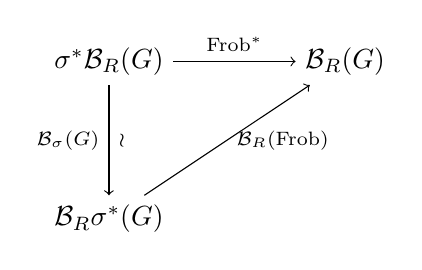
\begin{tikzpicture}
	\node (LT) at (0, 2) {$\sigma^*{\cal B}_R(G)$};
        \node (LB) at (0, 0) {${\cal B}_R\sigma^*(G)$};
	\node (RT) at (3, 2) {${\cal B}_R(G)$};
	\draw [->] (LT) -- node [left] {$\scriptstyle {\cal B}_\sigma(G)$} 
                           node [right] {$\scriptstyle \wr$} (LB);
	\draw [->] (LT) -- node [above] {$\scriptstyle \Frob^*$} (RT);
	\draw [->] (LB) -- node [right] {$\scriptstyle {\cal B}_R(\Frob)$} (RT);
  \end{tikzpicture}
  \end{center}
  commutes for all complete local rings $R$ containing ${\mb F}_p$ and 
  deformations $G$ of $\Gamma$ to $R$.  
 \end{enumerate}
 Morphisms in this category are maps of ring objects.  

 An object ${\cal B}$ is said to be {\em torsion free} if 
 ${\cal B}_R(G)$ is $p$-torsion free for every $p$-torsion free $R$ and 
 every deformation $G$ to $R$.  We denote by $\Alg_\DF^{\rm tf}$ the full subcategory of $\Alg_\DF$ consisting of torsion free objects.
\end{defn}

\begin{thm}[{\cite[pre-theorem 16.5]{lpo}}]
 There is a forgetful functor $\Model_{\DL_{E_0}} \to \Alg_\DF$ which 
 restricts to an equivalence $\Model_{\DL_{E_0}}^{\rm tf} \cong \Alg_\DF^{\rm tf}$ between the full subcategories of torsion 
 free objects.
\end{thm}


\subsection{Deformations of Frobenius are parametrized by subgroups}
\label{subsec:subgp}

Having identified the categories, we now analyze the essential data 
encoded in $\Mod_\DF$ and $\Alg_\DF^{\rm tf}$, by studying the structure of the 
category $\DF(R)$ of deformations of Frobenius.  This turns out to be 
parametrized by finite flat subgroups of the deformations of $\Gamma$ to $R$, as we explain below.

Choosing a coordinate of a formal group $G$ over $R$, a {\em degree} (or 
{\em rank}) {\em $d$ subgroup $K$ of $G$} is an effective divisor with 
$\CO_K = R \llbracket x \rrbracket / \big(f(x)\big)$ for some degree $d$ 
monic polynomial $f(x)$ such that 
$f(x_1 +_G x_2) \in \big(f(x_1),f(x_2)\big)$ 
and $f(x) \in (x)$.  In other words, the group law of $G$ restricts to 
$K$, and $K$ contains the identity.  Given a subgroup $K$ 
of $G$, we can define the {\em quotient group} $G/K$ (cf. \cite[section 5]{strick}) which is again a formal group.  

{\em Henceforth by ``subgroups'' we 
mean specifically those that are finite and flat.}  

One can show that the homomorphism $[d]_G\co G \to G$ restricts to zero 
on $K$ (cf. \cite[section 1]{tateoort}).  More concretely, this means that $f(x)$ 
must divide $[d]_G(x)$.  As a consequence, subgroups of a formal group 
over a $p$-local ring must have degree $p^r$.  In particular, if $G$ is a 
formal group over a field $k$ of characteristic $p>0$, there is exactly 
one subgroup of degree $p^r$, given by $f(x) = x^{p^r}$, which is the 
kernel of the $r$-fold Frobenius isogeny $\Frob^r$ (cf. \cite[proposition 16.8]{lpo}).  

We have seen that in $\DF(R)$ the degree 1 morphisms (when $r = 0$) 
are precisely the $\star$-isomorphisms of deformations.  In general, with morphisms corresponding to all 
$r \geq 0$, $\DF(R)$ is 
equivalent to the following category (cf. \cite[proposition 16.9]{lpo}).  
The objects are $\star$-isomorphism classes of deformations $[G]$.  The 
morphisms are $\star$-isomorphism classes of pairs $[G > K]$: the source 
of $[G > K]$ is $[G]$, and the target of $[G > K]$ is $[G/K]$, where 
$G/K$ is a deformation of $\Gamma$ with $i_{G/K} = \sigma^r \circ i_G$ 
($p^r$ being the degree of $K$).  Moreover, if $G/K \cong G'$, then 
$[G' > K'] \circ [G > K] = [G > K'']$, where $K''$ is the kernel of the 
composite $G \to G/K \cong G' \to G'/K'$.  Thus deformations of Frobenius 
with source $(G,i,\alpha)$ correspond {\em exactly} to subgroups of $G$.  

\begin{exam}
\label{ex:K}
Let $\Gamma$ be the multiplicative formal group over ${\mb F}_p$ 
of height 1.  For the multiplicative formal group $\Gm$ over a 
$p$-local ring $R$, since the formal group law is defined by 
$1 + (x_1 +_\Gm x_2) = (1 + x_1)(1 + x_2)$, we have 
$[p^r](x) = (1 + x)^{p^r} - 1 = x^{p^r}$.  Thus the only subgroups 
of $\Gm$ are $\Gm [p^r]$ with $\CO_{\Gm [p^r]} = \CO_\Gm / (x^{p^r})$.  
Moreover, by the Lubin-Tate theorem (cf. \cite[theorem 3.1]{lubintate} and \cite[section 4.3]{H-Mthm}), every object of $\DF(R)$ is 
$\star$-isomorphic to $\Gm$.  In particular, the set of 
$\star$-isomorphism classes of deformations of $\Gamma$ to $R$ 
is classified by the ring $\CO_{\rm univ} = {\mb Z}_p$, and we 
can take the universal deformation $G_{\rm univ}$ to be the 
multiplicative formal group over ${\mb Z}_p$.  Thus by functoriality, 
to describe an object ${\cal B} \in \Alg_\DF^{\rm tf}$, it is enough to give
\begin{enumerate}
\item a $p$-torsion free ${\mb Z}_p$-algebra $B = {\cal B}_{{\mb Z}_p}(\Gm)$, 
\item maps of ${\mb Z}_p$-algebras $\psi^{p^r}\co B \to B$ 
(corresponding to the isogenies $[p^r]\co \Gm \to \Gm$) such that 
\begin{enumerate}
 \item $\psi^1 = {\rm id}_B$ and $\psi^{p^r} \circ \psi^{p^s} = 
\psi^{p^{r+s}}$,
 \item $\psi^p(b) \equiv b^p$ mod $pB$.
\end{enumerate}
\end{enumerate}
(For comparison, the items are labelled as in definitions \ref{def:mod} and \ref{def:alg}.)  

We note as in \cite[example 1.3]{cong} that this is a 
``$p$-typicalization'' of the original theorem of Wilkerson 
(cf. \cite[proposition 1.2]{wilkerson}) which characterizes the torsion free $\lambda$-rings 
in terms of congruences on the Adams operations at all primes.  
More concretely, let $K$ be the complex $K$-theory spectrum.  Then for 
$B = \pi_0 A$, where $A$ is a $p$-complete $K$-algebra (commutative 
$K$-algebra such that $A \cong A_p^\wedge$), $\psi^p$ recovers the $p$'th 
Adams operation studied by McClure (cf. \cite[chapters VIII and IX]{BMSS}).  
\end{exam}

In general, consider the functor $X_r$ which associates to a ring $R$ the set of 
$\star$-isomorphism classes of pairs $[G > K]$ with $K$ a degree $p^r$ 
subgroup of $G$.  It is represented by the complete local ring $\CO_{X_r} = 
E^0 B\Sigma_{p^r}/I$, where $I = \sum_{0<i<p^r} 
{\rm Image}\big(E^0 B(\Sigma_i\times\Sigma_{p^r-i}) 
\xrightarrow{\text{transfer}} E^0 B\Sigma_{p^r}\big)$ is the 
{\em transfer ideal} (roughly speaking, the corresponding power operation 
should be additive, so modulo the ``mixing terms'' in the Cartan formula) (cf. \cite[theorem 9.2]{strickland}).  
This can be viewed as a generalization of the Lubin-Tate theorem for 
$\CO_{\rm univ} = \CO_{X_0}$.  Moreover, there are two ring homomorphisms 
$s^*$, $t^*\co \CO_{\rm univ} \to \CO_{X_r}$, where $s^*$ represents the 
source map $[G > K] \mapsto [G]$, and $t^*$ represents the target map 
$[G > K] \mapsto [G/K]$.  (In example \ref{ex:K}, 
$\CO_{X_r} \cong \CO_{\rm univ}$ for all $r$, and $s^* = t^* = 
{\rm id}$.)  Thus to describe an object ${\cal B} \in \Alg_\DF^{\rm tf}$, it is 
enough to give 
\begin{enumerate}
\item a $p$-torsion free $\CO_{\rm univ}$-algebra 
$B = {\cal B}_{\CO_{\rm univ}}(G_{\rm univ})$, 
\item maps of $\CO_{\rm univ}$-algebras 
$\psi^{p^r}\co B \to B \otimes_{\CO_{\rm univ}}^{s^*} \CO_{X_r}$ 
as the composite 
\[
 B \stackrel{f^*}{\to} B \otimes_{\CO_{\rm univ}}^{t^*} \CO_{X_r} 
\stackrel{{\cal B}_f}{\cong} {\cal B}_{\CO_{X_r}} (t^*G_{\rm univ}) 
\xrightarrow{{\cal B}_{\CO_{X_r}} (\psi)} {\cal B}_{\CO_{X_r}} (s^*G_{\rm univ}) 
\stackrel{{\cal B}_g}{\cong} B \otimes_{\CO_{\rm univ}}^{s^*} \CO_{X_r}, 
\]
where $f = t^*$ and $g = s^*$ are local homomorphisms, and 
$\psi\co s^*G_{\rm univ} \to t^*G_{\rm univ}$ is the 
universal deformation of $\Frob^r$ (cf. \cite[section 13]{strick}),
\end{enumerate}
satisfying a set of formal properties.  In particular, if we denote by 
$u^*$ the map $\CO_{X_1} \to \CO_{\rm univ}/(p)$ which represents the 
universal Frobenius isogeny, the Frobenius congruence (b) amounts to 
requiring that 
\[
 B \stackrel{\psi^p}{\to} B \otimes_{\CO_{\rm univ}}^{s^*} \CO_{X_1} 
\xrightarrow{{\rm id} \otimes u^*} B \otimes_{\CO_{\rm univ}} \CO_{\rm univ}/(p) 
= B/pB
\]
be the $p$'th power map $B \to B/pB \stackrel{\sigma}{\to} B/pB$ which sends $x$ to $\bar{x}^p$.  

\begin{exam}
\label{ex:h2p2}
Consider the elliptic curve $C_0 \subset {\mb P}_{{\mb F}_2}^2$ defined 
by
\[
 Y^2 Z + Y Z^2 = X^3,
\]
which is supersingular so that its formal group $\widehat{C_0}$ is of 
height 2.  It has a universal deformation $C$ over the Lubin-Tate ring 
${\mb W}{\mb F}_2 \llbracket v_1 \rrbracket \cong 
{\mb Z}_2 \llbracket a \rrbracket$ given by 
\[
 Y^2 Z + a X Y Z + Y Z^2 = X^3,
\]
where $a$ is the Hasse invariant so that setting $a=0$ we recover the 
supersingular elliptic curve $C_0$ (cf. \cite[2.2.10]{katzmazur} 
and \cite[proposition 3.2]{tmf3}).  Let $E$ be the Morava $E$-theory 
spectrum associated to this universal deformation, so that $\pi_* E = 
{\mb Z}_2 \llbracket a \rrbracket [v^{\pm 1}]$ with $|v| = 2$.  The power 
operations on $E$ are constructed in \cite[section 3]{Andu}, with explicit formulas 
computed in \cite[sections 3 and 4]{h2p2}.  What follows is directly from the latter reference.  

By studying degree 2 subgroups, i.e.\thinspace{s}ubgroups of 2-torsion 
points on $C$, we can identify $\CO_{X_1} \cong 
{\mb Z}_2 \llbracket a,d \rrbracket / (d^3 - a d - 2)$: in the affine 
chart $u = X/Y$, $v = Z/Y$, degree 2 subgroups are generated by points 
$Q$ of the form $\big(u(Q), v(Q)\big) = (d, -d^3)$ such that 
$d^3 - a d - 2 = 0$.  Thus we have a power operation 
\[
 \psi^2\co E^0 X \to E^0 X \llbracket d \rrbracket / (d^3 - a d - 2).
\]
Moreover, by studying the isogeny $\psi_Q\co C \to C'$ whose kernel is 
the degree 2 subgroup generated by $Q$, one computes that 
\[
 t^* (a) = \psi^2 (a) = a^2 + 3 d - a d^2.
\]
There are also formulas for a set of functions $Q_0(x)$, 
$Q_1(x)$ and $Q_2(x)$ which express
\[
 \psi^2 (x) = Q_0(x) + Q_1(x) d + Q_2(x) d^2.
\]
In particular, the Frobenius congruence takes the form 
$Q_0(x) \equiv x^2$ mod 2.  We will discuss in detail such calculations 
for Morava $E$-theories associated to supersingular elliptic curves in 
section \ref{sec:p3}.  
\end{exam}


\section{$K(1)$-local power operations}
\label{sec:K(1)}


In this section we discuss how to pass to the $K(1)$-local setting from 
the power operations at arbitrary height described in the previous 
section.  For general background of $K(1)$-local operations, see 
\cite{k1}.

Let $F$ be an even-periodic $E_\infty$ ring spectrum such that $F^0$ is a 
$p$-torsion free complete local ring with maximal ideal $\mf m$ 
containing $p$, and the mod-$\mf m$ reduction of the formal group over 
$F^0$ is of height $n < \infty$, and let $E = L_{K(1)} F$ be its 
$K(1)$-localization.  For example, the Morava $E$-theory spectrum 
associated to the universal deformation of a supersingular elliptic curve 
in example \ref{ex:h2p2} is such, and we write $F = E_2$, 
specifying its height.  

The general pattern of the relationship between $K(1)$-local power operations 
and the power operations in section \ref{subsec:subgp} is as follows: 
\begin{center}
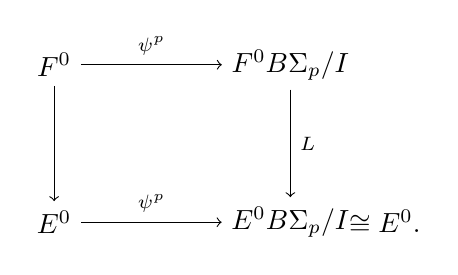
\begin{tikzpicture}
	\node (LT) at (0, 2) {$F^0$};
        \node (LB) at (0, 0) {$E^0$};
	\node (RT) at (3, 2) {$F^0 B\Sigma_p/I$};
	\node (RB) at (3, 0) {$E^0 B\Sigma_p/I$};
	\node at (4.2,0) {$\cong E^0.$}; 
	\draw [->] (LT) -- node [above] {$\scriptstyle \psi^p$} (RT); 
	\draw [->] (LB) -- node [above] {$\scriptstyle \psi^p$} (RB); 
	\draw [->] (LT) -- (LB); 
	\draw [->] (RT) -- node [right] {$\scriptstyle L$} (RB);
\end{tikzpicture}
\end{center}
Recall that the top operation arises from the universal deformation of 
Frobenius which is represented by the ring 
$\CO_{X_1} = F^0 B\Sigma_p/I$.  
The vertical maps are induced by the $K(1)$-localization $F \to E$.  In 
terms of homotopy groups, this is obtained by inverting the generator $v_1$ 
(so that the resulting formal group is of height at most 1) and 
completing at the ideal $(p)$, i.e.\thinspace
$F^0 = {\mb W}k \llbracket v_1,...,v_{n-1} \rrbracket$ and 
$E^0 = {\mb W}k \llbracket v_1,...,v_{n-1} \rrbracket [v_1^{-1}]_p^\wedge$.  
For example, $\pi_0 L_{K(1)} E_2 = \varprojlim {\mb Z_2} (\!(a)\!) /(2^i) = 
\{\sum_{n = -\infty}^{\infty} c_n a^n | c_n \in {\mb Z}_2, 
c_n \to 0 \text{~2-adically as~} n \to -\infty\}$ (the Hasse invariant $h = a$ can be taken as the generator $v_1$).  In particular the 
formal group of $F^0$ obtains a unique degree $p$ subgroup after being 
pulled back to $E^0$, and the map $L$ classifies it.  We will explain 
this uniqueness of subgroup and the isomorphism at the bottom right 
corner shortly.  

In order to do calculation we need to examine $L$ more carefully.  
For a $p$-divisible group $\mb G$ over a base scheme $X$, the restriction 
of $\mb G$ to any geometric point $x \in X$ lives in the natural short 
exact sequence 
\[
 0 \to \mb G^{\text{for}} \to \mb G_x \to \mb G^{\text{\'et}} \to 0,
\]
where the subobject (the connected component of the identity) is the 
{\em formal} component, and the quotient is the {\em \'etale} component.  The
formal component $\mb G^{\text{for}}$ is a formal group on $X$.  The 
localization $L$ factors through $E^0 \otimes_{F^0} F^0 B\Sigma_p/I$, and along the base change 
$F^0 B\Sigma_p/I \to E^0 \otimes_{F^0} F^0 B\Sigma_p/I$ the $p$-divisible 
group consisting solely of formal component may split into formal and 
\'etale components.  We want to take the formal component so as to keep track of the 
unique subgroup classified by $L$ which lands in the formal group over 
$E^0 B\Sigma_p/I$.  

\begin{exam}
\label{ex:h1p2}
We continue example \ref{ex:h2p2} in the $K(1)$-local setting.  After 
base change to $L_{K(1)} E_2$, the universal elliptic curve $C$ has a 
unique degree 2 subgroup in its formal component which is the canonical 
subgroup introduced in \cite[theorem 1.4]{lubin}.  The degree 2 
subgroup generated by $(d,-d^3)$ is contained in the formal component if 
and only if $(d,-d^3)$ is in the formal neighborhood of the identity 
$(0,0)$.  The equation $d^3 - a d - 2 = 0$ which parametrizes degree 2 
subgroups has a unique root in ${\mb F}_2 (\!(a)\!)$, and Hensel's lemma 
implies that this lifts to a root in 
$\pi_0 L_{K(1)} E_2 \cong {\mb Z}_2 (\!(a)\!)_2^\wedge$.  Plugging this specific 
value of $d$ into $\psi^2\co \pi_0 E_2 \to \pi_0 E_2 \llbracket d \rrbracket /(d^3-ad-2)$, we 
get an endomorphism of the ring $\pi_0 L_{K(1)} E_2$, and this 
endomorphism is the $K(1)$-local power operation.  For an application of 
this calculation, see \cite[section 6]{level3}.
\end{exam}

Lastly we note that the above commutative square describes the pattern 
for $K(m)$-local operations with $m > 1$ as well, but the isomorphism at 
the bottom right corner is specific to the height 1 case.  

\begin{lem}
\label{lem:cong}
$E^0 B\Sigma_p/I \cong E^0$.
\end{lem}
This generalizes what we have seen in 
example \ref{ex:K} about the multiplicative formal group.  A formal group 
$\mb G$ of height 1 has a unique degree $p$ subgroup given by 
${\mb G}[p]$, and the ring $E^0 B\Sigma_p/I$ classifying subgroups of 
degree $p$ is isomorphic to $E^0$.  Thus the power operation takes the 
form $\psi^p\co E^0 \to E^0$ which is a lift of Frobenius.  In general a 
height $n$ formal group has $(p^n-1)/(p-1)$ degree $p$ subgroups, as in 
the example of section \ref{sec:p3} where $n=2$ and $p=3$.  See \cite[section 3.5]{Andu} for an approach of making power operations of higher height land in $E^0$.  
\begin{proof}[Proof of the lemma]
First we identify $E^0 B\Sigma_p$ as the $E^0$-submodule of $E^0 BC_p$ fixed by 
the action induced by ${\rm Aut} C_p \cong {\mb F}_p^\times$. This is a 
special case of the calculation in \cite[section 12]{lpo}.  We have
\[
 B\Sigma_p \stackrel{\rm tr}{\longrightarrow} BC_p 
 \stackrel{\rm res}{\longrightarrow} B\Sigma_p,
\]
where $\rm tr$ is the transfer map, and $\rm res$ is the restriction map.  
Since $[\Sigma_p : C_p]$ is prime to $p$, the composite is a $p$-local 
equivalence, and thus $p$-locally $B\Sigma_p$ is a retract of $BC_p$.  
Moreover, ${\rm Aut} C_p$ acts on $\Hom (C_p,\Sigma_p)$ as conjugation (it preserves the ``cycle type'' of the element generating the image of $C_p$ in $\Sigma_p$).  
Thus two maps $C_p \to \Sigma_p$ that differ by an ${\rm Aut} C_p$-action induce homotopic maps $BC_p \to B\Sigma_p$, and hence the same map 
$E^0 B\Sigma_p \to E^0 BC_p$.  

We calculate $E^0 BC_p$ by considering 
the cofiber sequence associated to the construction of Thom space 
\[
 S(L^{\otimes p}) \to BS^1 \to (BS^1)^{L^{\otimes p}}, 
\]
where $L$ is the tautological complex line bundle over $BS^1$.  
$E^* BS^1$ can be calculated (cf. \cite[section 1]{coctalos}) as $E^0 \llbracket u \rrbracket$ with $|u| = 2$, 
where $u$ is the first Chern class of $L$.  By the Thom isomorphism and the even-periodicity of $E^*$, 
the map on cohomology induced by the right-hand map in the cofiber sequence can be identified as 
$[p]\co E^* BS^1 \to E^* BS^1$.  This map sends $u$ to $[p](u) = 
p u + \cdots + v_1 u^p + \cdots$, where $v_1$ is invertible in $E^0 \cong 
{\mb W}k \llbracket v_1,...,v_{n-1} \rrbracket [v_1^{-1}]_p^\wedge$.  
Also note that we can identify the sphere bundle $S(L^{\otimes p})$ with $BC_p$.  
Thus again as $E^*$ is even-periodic, the long exact sequence induced by the cofiber sequence implies that 
$E^0 BC_p \cong 
E^0 \llbracket u \rrbracket / \big([p](u)\big)$.  

For any $q \in {\mb F}_p^\times$, the induced action on $E^0 BC_p$ sends $u$ to 
$[q](u) = q u + \cdots$.  Hence as the $E^0$-submodule of $E^0 BC_p$ fixed by the ${\rm Aut} C_p$-action, $E^0 B\Sigma_p$ can be identified with 
$E^0 \oplus \big(E^0 \cdot \prod_{q=1}^{p-1} [q](u)\big) \cong E^0 \oplus \big(E^0 \cdot (u^{p-1} + \cdots)\big)$.  

Next we identify the transfer ideal $I = \sum_{0<i<p} 
{\rm Image}\big(E^0 B(\Sigma_i\times\Sigma_{p-i}) 
\xrightarrow{\text{transfer}} E^0 B\Sigma_{p}\big)$ as the second summand 
in $E^0 B\Sigma_p$.  Similarly as above, for all $0 < i < p$, the 
composite
\[
 E^0 B(\Sigma_i \times \Sigma_{p-i}) \stackrel{\rm res}{\longrightarrow} 
 E^0 \stackrel{\rm tr}{\longrightarrow} 
 E^0 B(\Sigma_i \times \Sigma_{p-i})
\]
is multiplication by an invertible scalar, and thus 
$E^0 B(\Sigma_i \times \Sigma_{p-i}) \cong E^0$.  Moreover, by the 
``double-coset formula'' the composite 
\[
 E^0 \stackrel{\rm tr}{\longrightarrow} E^0 B\Sigma_p 
 \stackrel{\rm res}{\longhookrightarrow} E^0 BC_p
\]
has image the same as $E^0 \stackrel{\rm tr}{\longrightarrow} E^0 BC_p$.  
Thus $I$ is generated by ${\rm tr}(1)$ as an $E^0$-module.  

Write $\langle p \rangle(u) = p + \cdots + v_1 u^{p-1} + \cdots$ so that $E^0 BC_p = E^0 \llbracket u \rrbracket / \big( u \cdot \langle p \rangle(u) \big)$, 
and write ${\rm tr}(1) = f(u) \in E^0 \llbracket u \rrbracket$ by abuse of 
notation.  Note that the composite 
\[
 E^0 \stackrel{\rm tr}{\longrightarrow} E^0 BC_p 
 \stackrel{\rm res}{\longrightarrow} E^0
\]
is multiplication-by-$p$.  Since this composite sends $1$ to ${\rm res}\big( f(u) \big) = f(0)$, we have $f(0) = p$.  
Moreover since $u \cdot {\rm tr}(1) = {\rm tr}\big( {\rm res}(u) \big)$ and ${\rm res}(u) = 0$, $u \cdot f(u)$ is divisible by $[p](u)$.  We claim that 
these two conditions on $f(u)$ forces it to be $\langle p \rangle (u)$.  Clearly $\langle p \rangle(0) = p$, and $\langle p \rangle(u)$ is annihilated by $u$ in $E^0 \llbracket u \rrbracket / \big( u \cdot 
\langle p \rangle(u) \big)$.  Applying the snake lemma to two rows of 
copies of
\[
 0 \longrightarrow E^0 \llbracket u \rrbracket 
 \stackrel{\cdot u}{\longrightarrow} E^0 \llbracket u \rrbracket 
 \longrightarrow E^0 \longrightarrow 0
\]
with vertical maps being multiplication by $[p](u)$ on 
$E^0 \llbracket u \rrbracket$ and zero on $E^0$, we see that any 
element annihilated by $u$ is a multiple of $\langle p \rangle(u)$ by an 
element of $E^0$.  As $p$ is not a zero-divisor in $E^0$, the claim 
follows.  Thus $I = E^0 \cdot \langle p \rangle(u)$.  

Finally as $v_1$ is invertible in $E^0$, $E^0 B\Sigma_p/I \cong E^0$.
\end{proof}

We also note that at height 1, as in example \ref{ex:K}, the power 
operation $\psi^p$ determines the other $\psi^{p^r}$ with 
$r > 1$ by iterated composition.  Thus in the $K(1)$-local setting, among the operations $\psi^{p^r}$ it suffices to study only $\psi^p$ as above.  
Moreover if the $K(1)$-local homotopy groups are {\em $p$-torsion free}, it turns out that $\psi^p$ determines {\em all} the power operations (cf. \cite[section 3]{lpo}).  For this reason 
we will simply write $\psi$ for {\em the} $K(1)$-local power operation.  
At higher height, the relationship among these operations is more 
complicated.  


\section{Power operations at the prime 3}
\label{sec:p3}


In \cite{h2p2}, Rezk gives explicit calculations of the algebraic theory 
of power operations for a specific Morava $E$-theory of height 2 at the 
prime 2 (cf. example \ref{ex:h2p2}).  We record some calculations 
mimicking some of the results there, at the prime 3, together with 
calculations of the corresponding $K(1)$-local power operation.  

The Morava $E$-theory $F$ of height 2 that we consider here is associated to 
the deformations of a supersingular elliptic curve over a field of characteristic 3.  Our 
calculations break into the following steps:
\begin{enumerate}
 \item Find the universal elliptic curve with a choice of 4-torsion 
 point, so that a posteriori the supersingular elliptic curve that we are 
 interested in is the one with the Hasse invariant zero; 
 \item Study the degree 3 subgroups of this universal elliptic curve.  In 
 particular, we need to compute 
\begin{itemize}
 \item the coordinate ring parametrizing degree 3 subgroups,  
 \item the equation of the quotient curve which is the image of the 
 universal degree 3 isogeny;
\end{itemize} 
 \item $K(1)$-localize.  
\end{enumerate}


\subsection{The universal elliptic curve with a choice of 4-torsion point}
\label{subsec:step1}

Let $k$ be a field of characteristic 3.  First we note that a 
supersingular elliptic curve over $k$ cannot have a 3-torsion point.  
Moreover, in order to have a {\em unique} lift of the elliptic curve together 
with a choice of $N$-torsion point along a deformation of $k$, $N$ must be 
prime to 3.  As the associated moduli stack 
${\cal M}\big(\Gamma_1(2)\big)$ to a level $\Gamma_1(2)$-structure on the 
elliptic curve is not representable by a scheme due to the existence of 
nontrivial automorphism of order 2 (cf. 
\cite[corollaries 4.7.2 and 2.7.2]{katzmazur}), a natural choice for 
the universal elliptic curve is one equipped with a level 
$\Gamma_1(4)$-structure.  

The computation for the equation of the universal elliptic curve with a 
choice of 4-torsion point $P$ is analogous to \cite[2.2.10]{katzmazur} 
and \cite[proposition 3.2]{tmf3}, where the universal elliptic curve for the prime 2 case has a choice of 3-torsion point (cf. example \ref{ex:h2p2}).  In the 
$xy$-coordinates, with the constraints that $P$ be at the origin, $2P$ be 
on the $x$-axis, and $4P$ be the identity $O$, we have the affine 
Weierstrass equation 
\[
 y^2 + a x y + a c y = x^3 + c x^2
\]
over the graded ring ${\mb Z}_{(3)}[a,c]$, where $|a| = 1$ and $|c| = 2$.  
The grading comes from the action of $\Gm = 
\Spec {\mb Z}[\lambda^{\pm1}]$ given by $a \mapsto \lambda a$ and 
$c \mapsto \lambda^2 c$.  By \cite[V.4.1(a)]{AEC}, the Hasse 
invariant can be computed as $h = a^2 + 4c$, so that over $k$ the curve 
is supersingular precisely when $h = 0$ (note that the minimal field of definition of this supersingular elliptic curve is ${\mb F}_9$).  To facilitate calculation, we 
work in the affine coordinate chart $c = 1$ of 
${\cal M}\big(\Gamma_1(4)\big)$ so that the elliptic curve is given by 
\[
 y^2 + a x y + a y = x^3 + x^2,
\]
with the discriminant of the elliptic curve $\Delta = a^2(a + 4)(a - 4)$ 
and the Hasse invariant $h = a^2 + 4$.  This reduction is analogous to 
the one discussed in detail in \cite[section 4]{level3}.  In the
$uv$-coodinates, with $u = x/y$ and $v = 1/y$, the equation becomes 
\[
 v + a u v + a v^2 = u^3 + u^2 v
\]
which is the form we will use most often later.  

We denote this elliptic curve by $\cal E$.  

\begin{rmk}
 We note that the curve $\cal E$, together with the universal elliptic curve with a choice of 
 3-torsion point for the prime 2 case, give models for studying power operations at
 {\em all} primes.  
\end{rmk}

As a record of notation, we can rewrite the equation of $\cal E$ as 
\[
 a v^2 + (1 + a u - u^2) v - u^3 = 0,
\]
and we denote by $\epsilon(v)$ the left-hand side of the above equation, viewed as a quadratic polynomial in $v$.  


\subsection{Degree 3 subgroups}
\label{subsec:step2}

\subsubsection{3-torsion points}
\label{subsec}

In order to compute the coordinate ring parametrizing degree 3 subgroups, we need to find an equation characterizing the coodinates of a 3-torsion point.  

Given the elliptic curve 
\[
 {\cal E}\co y^2 + a x y + a y = x^3 + x^2,
\]
$(x,y)$ is a 3-torsion point if and only if the division polynomial 
\[
 \psi_3 (x) = 3x^4 + (a^2 + 4) x^3 + 3a^2 x^2 + 3a^2 x + a^2 
\]
equals zero (cf. \cite[exercise 3.7(d)]{AEC}).  
(This polynomial is exactly what one gets for the characterization, away 
from the prime 2, of a flex point in terms of the second derivative $y''$ 
calculated by implicit differentiation.)  We want to translate this into 
the $uv$-coordinates which are more convenient to work with 
in the formal neighborhood of the identity (in the $xy$-coordinates, the 
identity is at $\infty$). In this way we will get a ``characteristic'' equation 
comparable to $d^3 - a d - 2 = 0$ in example \ref{ex:h2p2}, where $d$ was 
the $u$-coordinate of a 2-torsion point.  

From the formula of multiplication-by-3 in the $xy$-coordinates, we have
\[
 [3](u,v) = 
 \left(
 \frac{\phi_3(\frac{u}{v})\psi_3(\frac{u}{v})}{\omega_3(\frac{u}{v})},
 \frac{\psi_3(\frac{u}{v})^3}{\omega_3(\frac{u}{v})}\right),
\]
with notation following \cite[exercise 3.7(d)]{AEC}, and thus our 
preliminary equation is $\psi_3(\frac{u}{v}) = 0$.  Clearing the 
denominators in $\psi_3(\frac{u}{v})$ , we get 
\[
 \psi_3'(u,v) = 
 3u^4 + (a^2 + 4) u^3 v + 3a^2 u^2 v^2 + 3a^2 u v^3 + a^2 v^4.
\]
To eliminate $v$, we multiply the ``conjugate'' $\psi_3'(u,v')$, where 
$v$ and $v'$ are conjugate roots of the quadratic equation $\epsilon(v) = 0$.  We get a degree 8 polynomial in 
$u$:
\[
 f(u) = -3 - 3 a u + 8 u^2 - a^2 u^2 + 9 a u^3 - 6 u^4 + 6 a^2 u^4 + 
 7 a u^5 + a^3 u^5 + 3 a^2 u^6 + 3 a u^7 + u^8.
\]
Thus if we denote by $(d,e)$ the coordinates of a 3-torsion point, $d$ 
must satisfy $f(d) = 0$.  
\begin{rmk}
\label{rmk}
 According to section \ref{sec:K(1)}, in particular example 
 \ref{ex:h1p2}, we expect that $f(u)$ have a unique root reduced to zero 
 modulo 3 after $h = a^2 + 4$ gets inverted, corresponding to the unique 
 subgroup in the formal neighborhood of the identity.  However, as we obtain $f(u)$ out of a 
 conjugation procedure, this is not exactly the case.  We have 
 \[
  f(u) \equiv u^2 (u + a)^6~~\text{mod}~3,
 \]
 and in view of $a \not\equiv 0$ by the nonsingularity of $\cal E$ 
 (recall that $\Delta = a^2(a + 4)(a - 4)$), such a root has multiplicity 
 2 (corresponding to the two nontrivial elements in the subgroup).  
 $f(u)$ is the best possible polynomial solely about $u$ that we have at this 
 point, and in later steps we will have to ``rescale'' it 
 back to a degree 4 polynomial.  
\end{rmk}

Next, for the coordinates $(d,e)$ of a 3-torsion point, we want to 
express $e$ in terms of $d$.  At the prime 2 (cf. example \ref{ex:h2p2}), 
the relation $e = -d^3$ can be obtained by manipulating the 
division polynomial $\psi_2$ and its ``conjugate'' as above, or simply by 
computing the inversion formula for a 2-torsion point on the elliptic 
curve as in \cite[section 3]{h2p2}.  The prime 3 case is a little more involved.  

Using the Euclidean algorithm, we compute the gcd of 
\[
 A(v) = \psi_3'(u,v) = 3u^4 + (a^2 + 4) u^3 v + 3a^2 u^2 v^2 + 3a^2 u v^3 
 + a^2 v^4
\]
and 
\[
 B(v) = \epsilon(v),
\]
both of which vanish at $(d,e)$.  We have
\[
 A(v) = B(v)Q_1(v) + R_1(v)
\]
\[
 ~~~B(v) = R_1(v)Q_2(v) + R_2(v),
\]
and it turns out that $R_2(e) = 0$ as a result of $f(d) = 0$.  Thus
\[
 R_1(d,e) = p(d) + q(d) e = 0
\]
is a relation between $d$ and $e$, linear in $e$.  We have 
formulas for $p(d)$ and $q(d)$, and we can compute the inverse of $q(d)$ 
by applying the Euclidean algorithm to find 
\[
 1 = a(d)q(d) + b(d)f(d) = a(d)q(d).
\]
In the end we have a degree 7 polynomial $e = g(d)$, comparable to 
$e = -d^3$ in the prime 2 case.  

To summarize, in this subsection we find two polynomials $f$ and $g$, 
so that any 3-torsion point with the $uv$-coordinates $(d,e)$ satisfies 
$f(d) = 0$ and $e = g(d)$.  


\subsubsection{The universal degree 3 isogeny}

Now we are ready to compute the universal degree 3 isogeny and thus the 
equation of the quotient curve which is its image. From there we can find a 
formula for the power operation 
$\psi^3\co F^0  \to F^0 \llbracket d \rrbracket / \big(f(d)\big)$, where $F^0 = 
{\mb Z}_9 \llbracket h \rrbracket$ with the Hasse invariant $h$ as the generator $v_1$ (to be precise, the target should 
actually be a certain improved coordinate ring as promised in remark \ref{rmk}).  

To compute the coordinates $(u',v')$ 
of the isogeny, we follow the ``Lubin isogeny'' construction (cf. 
\cite[proof of theorem 1.4]{lubin}).  Let $P\big(u,v(u)\big)$ be a general point on 
$\cal E$, and $Q\big(d,e(d)\big)$ be a 3-torsion point.  For $v(u)$, we solve the quadratic equation $\epsilon(v) = 0$, and take 
the first few terms (up to at least $u^9$ for 
our purpose) in the power series expansion of the root satisfying $v(0)=0$ (lying in the formal neighborhood of the identity).  
For $e(d)$, we use the polynomial $g(d)$ computed at the end of section \ref{subsec}.  We set 
\[
 u' = u(P) u(P-Q) u(P+Q),
\]
and similarly for $v'$.  By computing the inversion and addition formulas 
for the curve $\cal E$, we can write down formulas for $u' = 
\alpha u + \cdots$ and $v' = \beta u^3 + \cdots$ in terms of the 
uniformizer $u$ and parameters $a$ and $d$.  
\begin{rmk}
 In order to have the equation of the quotient curve in Weierstrass form, 
 we need to include an adjusting constant factor $\alpha^3 / \beta$ into 
 $v'$, comparable to the term $-1$ appearing in the formula for $u'$ in 
 \cite{h2p2}.  
\end{rmk}
We then solve for the Weierstrass equation which $u'$ and $v'$ satisfy.  The equation of the quotient curve turns out to be 
\[
 v + r u v + r v^2 = u^3 + u^2 v,
\]
where

$r(a,d) = -\frac{1}{(-4 + a) (4 + a)}(-126 a + 28 a^3 - a^5 + 120 d - 
9 a^2 d + 3 a^4 d + 258 a d^2 - 67 a^3 d^2 + 3 a^5 d^2 - 152 d^3 + 
208 a^2 d^3 - 40 a^4 d^3 + a^6 d^3 + 198 a d^4 - 33 a^3 d^4 - 
3 a^5 d^4 + 8 d^5 + 63 a^2 d^5 - 15 a^4 d^5 + 70 a d^6 - 17 a^3 d^6 + 
24 d^7 - 6 a^2 d^7)$

(note that $(-4 + a) (4 + a)$ is invertible as $\Delta = 
a^2(a + 4)(a - 4)$).  Hence $\psi^3(a) = r(a,d)$ gives the power 
operation.  As $d \equiv 0$ mod 3, we check that $\psi(a)$ reduces to $a^3$ modulo 3 (the Frobenius 
congruence at height 1 over $k$).  

Lastly we compute the coordinate ring as the target of the power 
operation $\psi^3$.  

Set $t = g(d)/d$, the reciprocal of the 
$x$-coordinate of a 3-torsion point.  This is a quantity which is 
invariant under negation using the group law of $\cal E$ (as we have 
$[-1](x) = x$) and is ``distinguishable'' from the identity in the formal 
neighborhood (in the $xy$-coodinates the identity is at $\infty$).  In view of 
$f(d) = 0$, we compute that $t$ is the root of a quartic polynomial 
\[
 w(t) = a^2 t^4 + 3 a^2 t^3 + 3 a^2 t^2 + (a^2 + 4) t + 3
\]
which has a {\em unique} root reduced to zero modulo 3.  We note that via the 
relation $t = 1/x$ this polynomial recovers the division polynomial 
$\psi_3(x)$.  Thus the eight roots of $f(d)$ together with $d = 0$ 
correspond to the nine 3-torsion points on $\cal E$, and the four roots 
of $w(t)$ correspond to the four degree 3 subgroups consisting of 
3-torsion points, one of which lies in the formal neighborhood of the 
identity.  In particular, the equation of $\cal E$ implies that $d$ 
satisfies a quadratic equation in terms of $t$: 
\[
 (t + 1) d^2 - a t (t + 1) d - t = 0.
\]
From this equation and $w(t) = 0$, we can rewrite $\psi^3(a) = r(a,d)$ 
above in terms of $t$.  

The above calculations are summarized as follows.  
\begin{prop}
 The universal degree 3 isogeny with source $\cal E$ is defined over the 
 ring $F^0 \llbracket t \rrbracket / \big(a^2 t^4 + 3 a^2 t^3 + 3 a^2 t^2 + 
 (a^2 + 4) t + 3\big)$, and has target the elliptic curve 
 \[
  y^2 + r x y + r y = x^3 + x^2,
 \]
 where $r(a,t) = a^3 t^3 + 3 a^3 t^2 + 3 a^3 t - 4 a t + a^3 - 3 a$.  The 
 kernel of this isogeny is generated by the 3-torsion point with 
 $x$-coordinate $1/t$.  Thus the power operation $\psi^3$ is given by 
 
 $\psi^3(h) = (t + 1)^3 h^3 - (22 t^3 + 69 t^2 + 75 t + 27) h^2 + 
 (128 t^3 + 424 t^2 + 512 t + 201) h - 16 (14 t^3 + 49 t^2 + 65 t + 27)$, 

 $\psi^3(a) = (t + 1)^3 a^3 - (4 t + 3) a$.  
\end{prop}
\begin{rmk}
 Recall that $F^0 = 
{\mb Z}_9 \llbracket h \rrbracket$.  In the above we also give the formula for $\psi(a)$ since $a \in F^0$.  
In fact, we have 
\[
 a^2 = h - 4 \equiv -1~~\text{mod}~(3,h),
\]
where the ideal $(3,h)$ is prime in ${\mb Z} [h]$.  Thus by Hensel's lemma, $a - i \in {\mb Z}_3 \llbracket h \rrbracket$, where $i^2 + 1 = 0$.  But $i$ 
generates ${\mb Z}_9$ over ${\mb Z}_3$.  
\end{rmk}  


\subsection{$K(1)$-localize}
\label{subsec:step3}

As in example \ref{ex:h1p2}, with $h = a^2 + 4$ invertible, we can 
solve for $t$ 3-adically from the equation $w(t) = 0$ by first writing 
\[
 t = -\frac{1}{a^2 + 4}(a^2 t^4 + 3 a^2 t^3 + 3 a^2 t^2 + 3),
\]
and then substituting $t$ recursively.  Plugging this uniquely determined 
value of $t$ into $\psi^3(h,t)$ computed above, 
we get the $K(1)$-local power operation $\psi$ as an endomorphism of the 
ring $E^0 = {\mb Z}_9 (\!(h)\!)_3^\wedge$.  


\nocite{*}
\bibliographystyle{amsalpha}
\bibliography{po}
\end{document}
